\section{Segment trees for stabbing queries}
\label{sec:segmenet-trees}

Consider the set of line segments $L = \{ \ell_1, \ell_2, \ell_3, \ell_4, \ell_5\}$ in the following diagram: 

\begin{figure}[h!]
\centering
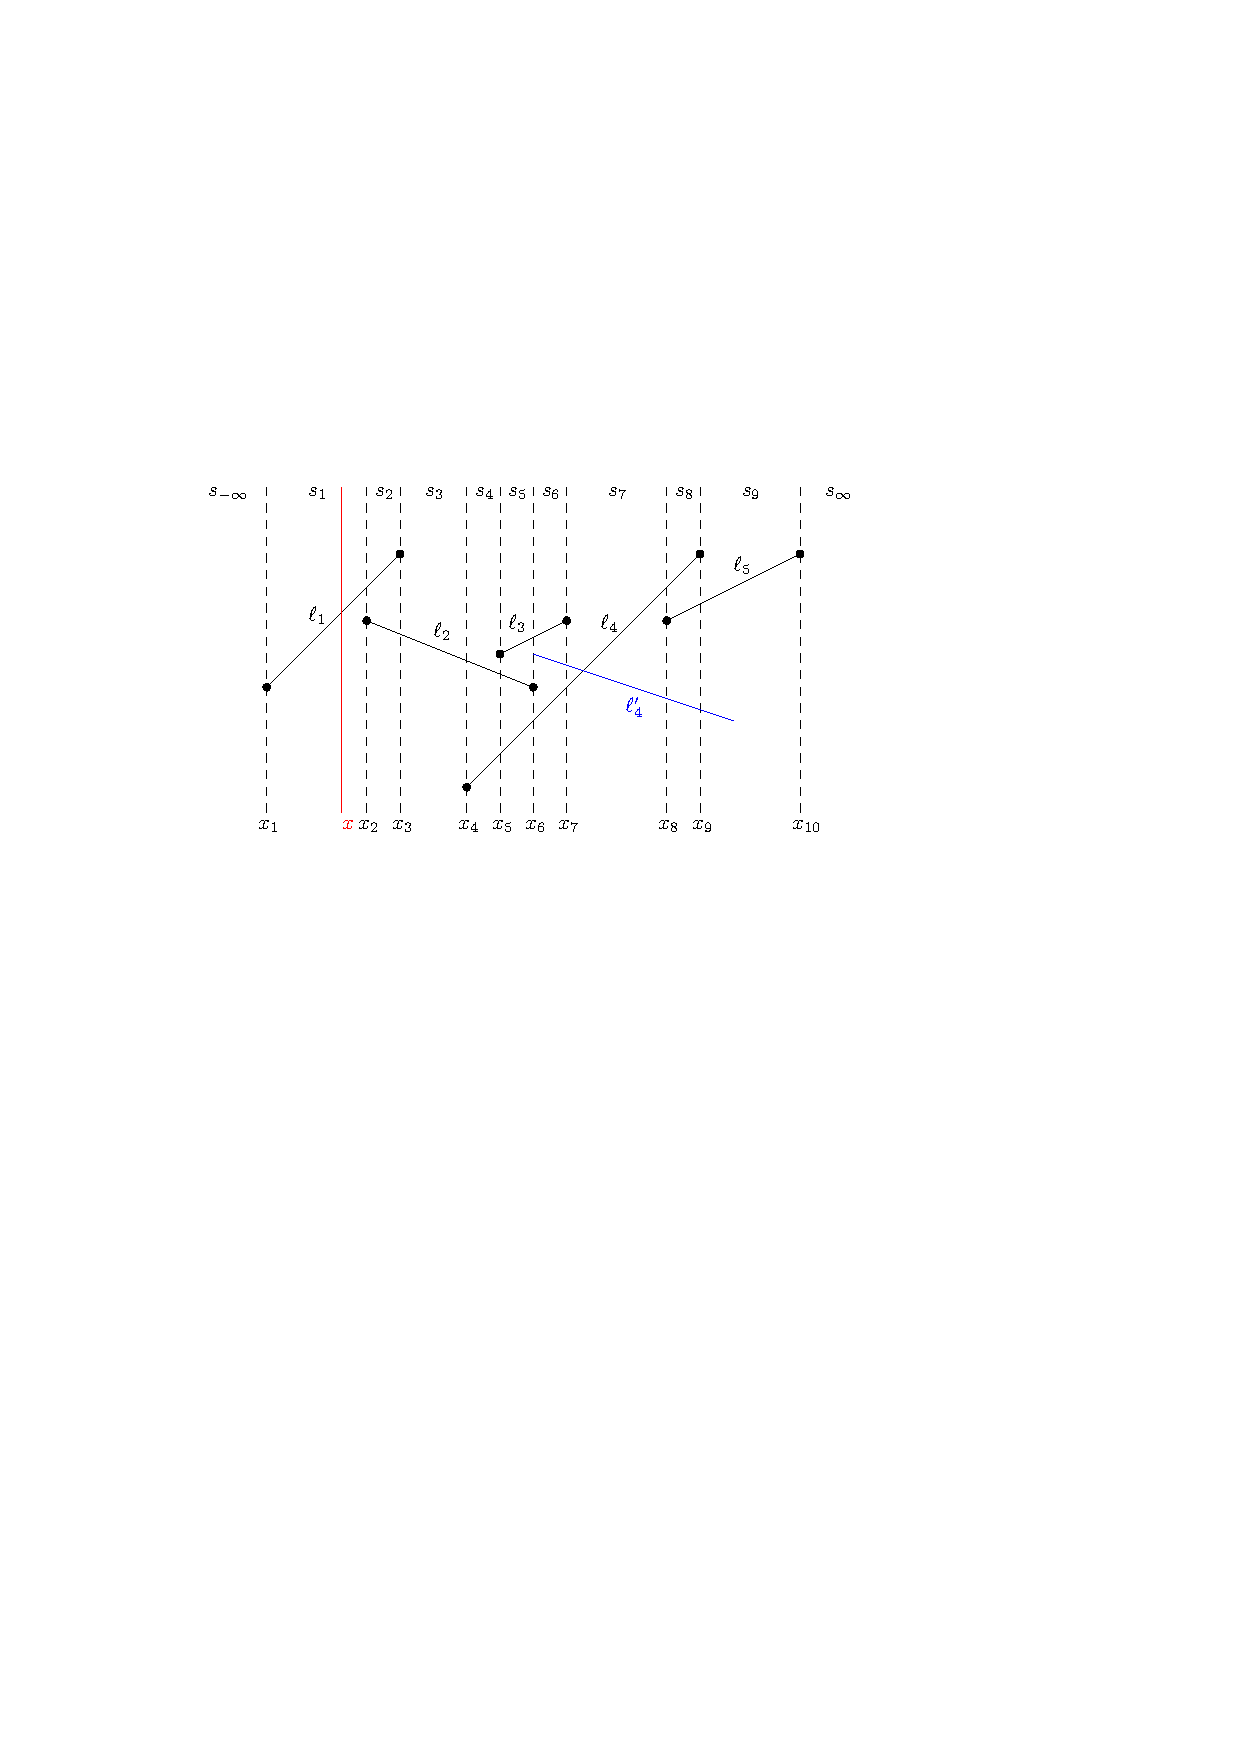
\includegraphics[scale = .8]{ipe/slanted-lines.pdf}
\caption{Set of line segments $L = \{ \ell_1, \ell_2, \ell_3, \ell_4, \ell_5\}$ with slabs $S = \{s_{-\infty},s_1, \dots, s_9, s_{\infty} \}$.}
\end{figure}
Observe that we cannot always define a total ordering over slanted line segments that preserves the transitivity property. 
%
For example, if we consider $\ell_5 \leq \ell_4 \leq \ell_2$ then by transitivity we would have $\ell_5 \leq \ell_2$. 
%
On the other hand, if we consider $\ell_2 \leq \textcolor{red}{\ell'_4} \leq \ell_5$ then we would have $\ell _2 \leq \ell_5$. 
%
However, if we divide the plane into slabs shown by the dashed lines, we can define a total ordering within each slab that is transitive. 

We can build a BST for slabs based on $x$-values of end points with leaves $S = \{s_{-\infty},s_1, \dots, s_9, s_{\infty} \}$, and internal node $v$ being the union of all slabs within the subtree rooted at $v$. 
%
The root is then all $x$-axis given by the only slab $[-\infty, \infty]$.
%
Next we augment the BST node $v$ with list of line segments $\ell$ that crosses any slab with its subtree but do not cross the parent slab. 
%
\paragraph{Invariant} Each line segment $\ell$ is stored in a node of $v$ such that 
\[ [v.x_{left}, v.x_{right}] \subseteq [ \ell.x_{left}, \ell.x_{right}]   \; \wedge \; [parent(v).x_{left}, parent(v).x_{right}] \not \subseteq [\ell.x_{left}, \ell.x_{right}].   \]

\begin{claim}
Each segment will be stored in at most 2 nodes at each level of segment tree.
\end{claim} 

The proof of the claim above can be found in chapter 10 in \cite{Berg:2008}. Based on the result above, the segment tree would take $O(n \log n)$ space and answer stabbing queries in $O(\log n + k)$.